\documentclass[aspectratio=169, 12pt]{beamer}

% =================== PRESENTER MODE TOGGLE ===================
% Define \presentermode (via Makefile) to produce a wide PDF with
% slide + notes side-by-side, consumable by pdfpc's presenter view.
%   Conference (clean):    make slides.pdf
%   Practice / recording:  make slides-presenter.pdf && pdfpc slides-presenter.pdf
\ifdefined\presentermode
  \setbeameroption{show notes on second screen=right}
  % Use the plain template -- drops the redundant slide thumbnail and
  % header, giving the notes panel ~30% more vertical room.
  \setbeamertemplate{note page}[plain]
  \setbeamerfont{note page}{size=\footnotesize}
  \setbeamerfont{note title}{size=\small, series=\bfseries}
\fi

% =================== THEME & GENERAL SETUP ===================
\usetheme{Boadilla}
\usecolortheme{whale}
\setbeamertemplate{navigation symbols}{}

% Footline with frame numbering (respects [noframenumbering])
\setbeamertemplate{footline}{%
  \leavevmode%
  \hbox{%
    \begin{beamercolorbox}[wd=\paperwidth,ht=2.25ex,dp=1ex,right]{date in head/foot}%
      \usebeamerfont{date in head/foot}\insertframenumber{} / \inserttotalframenumber\hspace*{2ex}
    \end{beamercolorbox}}%
  \vskip0pt%
}

% =================== PACKAGES ===================
\usepackage{graphicx}
\usepackage{tikz}
\usepackage{booktabs}
\usepackage{amsmath,amssymb}
\usepackage{fontawesome5}
\usepackage{colortbl}
\usepackage{tcolorbox}
\usepackage{lmodern}

\usetikzlibrary{shadows, calc, shapes, positioning, shadows.blur,
                decorations.pathreplacing, fadings, backgrounds, fit, arrows.meta}

% Path to paper figures
\graphicspath{{../../experiments/figures/}{./images/}}

% =================== COLOR PALETTE (matches prior deck for series identity) ===================
\definecolor{PrimaryBlue}{RGB}{0, 82, 155}
\definecolor{AccentOrange}{RGB}{230, 97, 0}
\definecolor{TheoreticalBlue}{RGB}{52, 152, 219}
\definecolor{PracticalGreen}{RGB}{46, 204, 113}
\definecolor{BridgeTeal}{RGB}{22, 160, 133}
\definecolor{HippoPurple}{RGB}{142, 68, 173}
\definecolor{NeoGold}{RGB}{211, 159, 39}
\definecolor{ShadowGray}{RGB}{189, 195, 199}
\definecolor{BackgroundLight}{RGB}{250, 250, 250}

\setbeamercolor{structure}{fg=PrimaryBlue}
\setbeamercolor{frametitle}{bg=PrimaryBlue!8, fg=PrimaryBlue}
\setbeamercolor{block title}{bg=PrimaryBlue!15, fg=PrimaryBlue}
\setbeamercolor{block body}{bg=PrimaryBlue!5}
\setbeamercolor{block title example}{bg=PracticalGreen!20, fg=PracticalGreen!80!black}
\setbeamercolor{block body example}{bg=PracticalGreen!5}
\setbeamercolor{block title alerted}{bg=AccentOrange!20, fg=AccentOrange!80!black}
\setbeamercolor{block body alerted}{bg=AccentOrange!5}

\setbeamertemplate{itemize items}[circle]
\setbeamertemplate{itemize item}{\small\textcolor{PrimaryBlue}{\textbullet}}
\setbeamertemplate{itemize subitem}{\tiny\textcolor{PrimaryBlue!70}{$\blacktriangleright$}}

% =================== TITLE METADATA ===================
\title[Episodes to Abstractions]{From Episodes to Abstractions}
\subtitle{Latent Hierarchical Memory in 1{,}908 AI Conversations}
\author{Alex Towell \and John Matta}
\institute[SIUE]{Southern Illinois University Edwardsville}
\date{ISCS 2026}

\begin{document}

% =====================================================================
% 1. TITLE
% =====================================================================
\begin{frame}[plain]
    \begin{tikzpicture}[remember picture, overlay]
        \fill[PrimaryBlue!5] (current page.north west) rectangle (current page.south east);
        \fill[PrimaryBlue] (current page.north west) rectangle ([yshift=-0.25cm]current page.north east);
        \fill[ShadowGray, opacity=0.08] ([yshift=1.5cm]current page.south west) rectangle (current page.south east);
        % ISCS 2026 conference logo (required on first slide).
        % Placed at bottom-right corner because the conference rule
        % requires the recorded speaker headshot to live in the
        % top-right -- the logo would be obscured if placed there.
        \node[anchor=south east, inner sep=0pt]
            at ([xshift=-0.6cm, yshift=0.3cm]current page.south east) {%
            \IfFileExists{images/iscs2026-logo.png}{%
                
\includegraphics[height=1.4cm]{images/iscs2026-logo.png}%
            }{\IfFileExists{images/iscs2026-logo.pdf}{%
                
\includegraphics[height=1.4cm]{images/iscs2026-logo.pdf}%
            }{\fbox{\parbox{2.4cm}{\centering\scriptsize\color{black!50}%
                ISCS 2026\\logo\\\textit{(missing)}}}}}%
        };
    \end{tikzpicture}

    \setlength{\columnsep}{18pt}
    \begin{columns}[T]
        \column{0.62\textwidth}
        \vspace{1.0cm}

        {\fontsize{22}{26}\selectfont\textcolor{PrimaryBlue}{\textbf{From Episodes to Abstractions}}}\\[0.3cm]
        {\large\textcolor{black!75}{Latent Hierarchical Memory in 1{,}908 AI Conversations}}\\[0.9cm]

        {\large\textbf{Alex Towell} \quad \textbf{John Matta}}\\[0.15cm]
        {\normalsize\textit{Southern Illinois University Edwardsville}}\\[0.10cm]
        {\normalsize\texttt{\textcolor{PrimaryBlue}{\{atowell, jmatta\}@siue.edu}}}\\[1.0cm]

        {\footnotesize\faGithub\ \textcolor{PrimaryBlue}{\url{github.com/queelius/chatgpt-complex-net}}}\\[0.1cm]
        {\footnotesize\textit{ISCS 2026 -- La Rochelle, France}}

        \column{0.38\textwidth}
        \vspace{0.5cm}
        \centering
        % Hierarchy schematic: episodes -> meta-concepts -> themes -> domains
        
\begin{tikzpicture}[scale=0.7, transform shape]
            % Outer ring: episodes (many dots)
            \foreach \a in {0,12,...,348} {
                \fill[PrimaryBlue!30] (\a:2.4) circle (0.05);
            }
            % Mid-outer ring: meta-concepts
            \foreach \a in {0,18,...,342} {
                \fill[TheoreticalBlue!70] (\a:1.7) circle (0.08);
            }
            % Mid-inner ring: themes
            \foreach \a in {0,36,...,324} {
                \fill[BridgeTeal!80] (\a:1.05) circle (0.11);
            }
            % Inner ring: 8 domains
            \foreach \a/\c in {0/AccentOrange, 45/PrimaryBlue, 90/PracticalGreen,
                               135/HippoPurple, 180/NeoGold, 225/TheoreticalBlue,
                               270/BridgeTeal, 315/AccentOrange!70} {
                \fill[\c] (\a:0.45) circle (0.17);
            }
        \end{tikzpicture}

        \vspace{0.2cm}
        % Legend reads outside-in to match the ring stack: outer to inner =
        % episodes -> meta-concepts -> themes -> domains.
        {\footnotesize
        \begin{tabular}{@{}r@{\hspace{4pt}}l@{}}
            \textcolor{PrimaryBlue!50}{$\bullet$} & outer:\ \ 1{,}908 episodes \\
            \textcolor{TheoreticalBlue}{$\bullet$} & \phantom{outer:\ \ }500 meta-concepts \\
            \textcolor{BridgeTeal}{$\bullet$} & \phantom{outer:\ \ }50 themes \\
            \textcolor{AccentOrange}{$\bullet$} & inner:\ \ 8 domains \\
        \end{tabular}
        }
    \end{columns}

    \note{%
        \textbf{Slide 1 -- Title (35 s, $\sim$85w)}\\[2pt]
        Good afternoon. I'm Alex Towell. Joint work with John Matta at SIUE.\\[2pt]
        In the last three years, millions of people have had thousands of conversations
        with LLMs. Each one is a trace of an idea being explored. What if we treated
        these archives not as chat logs, but as externalised semantic memory?\\[2pt]
        That's the question this paper asks. I'll show that one user's 1{,}908 ChatGPT
        conversations contain the same kind of structure cognitive scientists find in
        human semantic memory.\\[2pt]
        \textit{[Advance.]}
    }
\end{frame}

% =====================================================================
% 2. THE PROBLEM -- archives as flat lists hide the structure
% =====================================================================
\begin{frame}{The Problem: Archives Are Flat. Knowledge Is Not.}
    \begin{columns}[T]
        % LEFT: the scroll
        \column{0.30\textwidth}
        \centering
        \textbf{\textcolor{gray}{What you have}}\\[0.15cm]
        {\scriptsize \textit{Chronological list}}

        \vspace{0.25cm}
        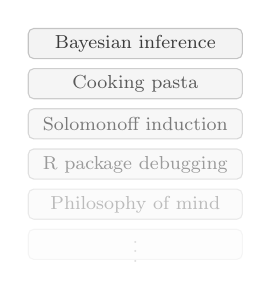
\begin{tikzpicture}[scale=0.85, transform shape]
            \foreach \y/\op/\lbl in {2.4/0.9/{Bayesian inference},
                                     1.8/0.75/{Cooking pasta},
                                     1.2/0.6/{Solomonoff induction},
                                     0.6/0.45/{R package debugging},
                                     0.0/0.3/{Philosophy of mind},
                                     -0.6/0.15/{$\vdots$}} {
                \draw[draw=gray!50, fill=gray!10, opacity=\op, rounded corners=2pt]
                    (-1.6, \y) rectangle (1.6, \y+0.45);
                \node[font=\footnotesize, opacity=\op, gray!30!black] at (0, \y+0.22) {\lbl};
            }
        \end{tikzpicture}

        \vspace{0.2cm}
        {\scriptsize \textcolor{AccentOrange!80!black}{\textit{Structure is invisible.}}}

        % MIDDLE: the transformation
        \column{0.40\textwidth}
        \centering
        \vspace{0.3cm}

        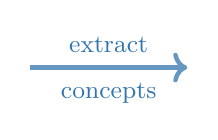
\begin{tikzpicture}
            \draw[->, ultra thick, PrimaryBlue!60] (-1, 0) -- (1, 0);
            \node[font=\small, text=PrimaryBlue!80, above=2pt] at (0, 0) {extract};
            \node[font=\small, text=PrimaryBlue!80, below=2pt] at (0, 0) {concepts};
        \end{tikzpicture}

        \vspace{0.3cm}

        \begin{block}{The Question}
            \footnotesize
            Does \textbf{structure} emerge from a long archive of AI
            conversations~--- the way it does in human memory?
        \end{block}

        % RIGHT: the structure
        \column{0.30\textwidth}
        \centering
        \textbf{\textcolor{PrimaryBlue}{What's hidden}}\\[0.15cm]
        {\scriptsize \textit{Latent hierarchy}}

        \vspace{0.25cm}
        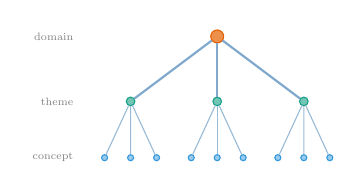
\begin{tikzpicture}[scale=0.55, transform shape]
            % Tree-style: 1 root, 3 branches, 9 leaves
            \node[circle, fill=AccentOrange!70, draw=AccentOrange, inner sep=3pt] (r) at (0, 3.2) {};
            \foreach \x/\name in {-2/a, 0/b, 2/c} {
                \node[circle, fill=BridgeTeal!60, draw=BridgeTeal, inner sep=2pt] (\name) at (\x, 1.7) {};
                \draw[PrimaryBlue!50, thick] (r) -- (\name);
            }
            \foreach \px/\name in {-2.6/a1, -2/a2, -1.4/a3,
                                   -0.6/b1, 0/b2, 0.6/b3,
                                   1.4/c1, 2/c2, 2.6/c3} {
                \node[circle, fill=TheoreticalBlue!50, draw=TheoreticalBlue, inner sep=1.4pt] (\name) at (\px, 0.4) {};
            }
            \draw[PrimaryBlue!40] (a) -- (a1); \draw[PrimaryBlue!40] (a) -- (a2); \draw[PrimaryBlue!40] (a) -- (a3);
            \draw[PrimaryBlue!40] (b) -- (b1); \draw[PrimaryBlue!40] (b) -- (b2); \draw[PrimaryBlue!40] (b) -- (b3);
            \draw[PrimaryBlue!40] (c) -- (c1); \draw[PrimaryBlue!40] (c) -- (c2); \draw[PrimaryBlue!40] (c) -- (c3);

            \node[font=\scriptsize, gray, anchor=east] at (-3.2, 3.2) {domain};
            \node[font=\scriptsize, gray, anchor=east] at (-3.2, 1.7) {theme};
            \node[font=\scriptsize, gray, anchor=east] at (-3.2, 0.4) {concept};
        \end{tikzpicture}

        \vspace{0.05cm}
        {\scriptsize \textcolor{PracticalGreen!70!black}{\textit{If it's there, we should find it.}}}
    \end{columns}

    \note{%
        \textbf{Slide 2 -- The Problem (50 s, $\sim$115w)}\\[2pt]
        \textit{[Gesture: left panel.]} When you open your ChatGPT history, you see
        this: a chronological list. Bayesian inference next to cooking pasta next to
        Solomonoff induction. Adjacency in \emph{time} tells you nothing about which
        conversations are about the same \emph{thing}.\\[2pt]
        \textit{[Gesture: right panel.]} But you know structure is there. You came
        back to Solomonoff three times last month; Bayesian inference is part of a
        domain you've been exploring. The hierarchy on the right is real --- it's
        just invisible from a list.\\[2pt]
        So: can we recover that structure automatically? And is it the kind of
        structure cognitive science predicts for semantic memory?\\[2pt]
        To answer that, I borrow a framework from a different field.
    }
\end{frame}

% =====================================================================
% 3. COGNITIVE FRAMEWORK
% =====================================================================
\begin{frame}{Two Ideas from Cognitive Science}
    \begin{columns}[T]
        % LEFT: CLS schematic
        \column{0.50\textwidth}
        \centering

        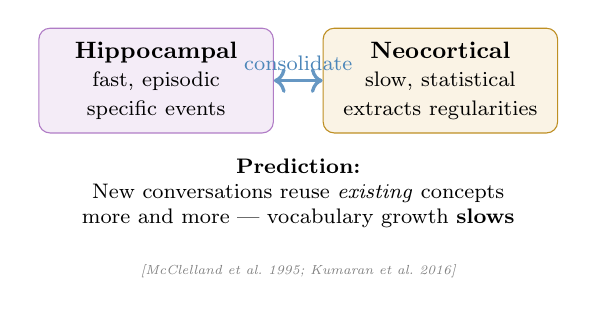
\begin{tikzpicture}[scale=0.95, transform shape]
            % Two coupled systems
            \node[draw=HippoPurple!70, fill=HippoPurple!10, rounded corners=4pt,
                  text width=2.9cm, align=center, font=\small, minimum height=1.4cm] (h)
                at (-1.9, 0) {\textbf{Hippocampal}\\[1pt]\footnotesize fast, episodic\\specific events};
            \node[draw=NeoGold!90!black, fill=NeoGold!12, rounded corners=4pt,
                  text width=2.9cm, align=center, font=\small, minimum height=1.4cm] (n)
                at (1.9, 0) {\textbf{Neocortical}\\[1pt]\footnotesize slow, statistical\\extracts regularities};
            % Bi-directional arrow
            \draw[<->, line width=1.2pt, PrimaryBlue!60] (h) -- (n)
                node[midway, above, font=\footnotesize, text=PrimaryBlue!70] {consolidate};

            % Below: prediction
            \node[font=\footnotesize, align=center, text width=7cm] at (0, -1.5) {%
                \textbf{Prediction:}\\
                New conversations reuse \emph{existing} concepts\\
                more and more~--- vocabulary growth \textbf{slows}};
            \node[font=\tiny\itshape, color=gray, align=center] at (0, -2.55)
                {[McClelland et al.\ 1995; Kumaran et al.\ 2016]};
        \end{tikzpicture}

        % RIGHT: semantic memory networks
        \column{0.50\textwidth}
        \centering

        \textbf{And: human semantic memory is}\\\textbf{a small-world network}

        \vspace{0.1cm}

        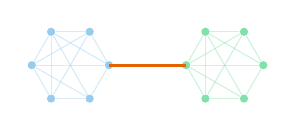
\begin{tikzpicture}[scale=0.7, transform shape]
            % Two clusters connected by a long-range edge
            \begin{scope}[shift={(-1.4, 0)}]
                \foreach \a in {0,60,...,300} {
                    \node[circle, fill=TheoreticalBlue!50, inner sep=1.5pt] (l\a) at (\a:0.7) {};
                }
                \foreach \a/\b in {0/60, 60/120, 120/180, 180/240, 240/300, 300/0,
                                   0/120, 60/180, 120/240, 180/300, 0/180, 60/240, 120/300} {
                    \draw[TheoreticalBlue!50, opacity=0.4] (l\a) -- (l\b);
                }
            \end{scope}
            \begin{scope}[shift={(1.4, 0)}]
                \foreach \a in {0,60,...,300} {
                    \node[circle, fill=PracticalGreen!60, inner sep=1.5pt] (r\a) at (\a:0.7) {};
                }
                \foreach \a/\b in {0/60, 60/120, 120/180, 180/240, 240/300, 300/0,
                                   0/120, 60/180, 120/240, 180/300, 0/180, 60/240, 120/300} {
                    \draw[PracticalGreen!60, opacity=0.4] (r\a) -- (r\b);
                }
            \end{scope}
            % Long-range shortcut
            \draw[AccentOrange, very thick] (-0.7, 0) -- (0.7, 0);
        \end{tikzpicture}

        \vspace{0.05cm}
        {\footnotesize Dense local clusters + a few global shortcuts.\\
        Roget's, WordNet, word associations: \textcolor{PrimaryBlue!80}{\textbf{small-worldness $\approx 5$--$15$}}}\\[1pt]
        {\tiny\itshape\color{gray} [Steyvers \& Tenenbaum 2005]}
    \end{columns}

    \vspace{0.25cm}

    \begin{alertblock}{The Hypothesis}
        \centering
        \small
        If AI conversation archives are an \emph{externalised} semantic memory,
        we should see both signatures:
        \textbf{sublinear vocabulary growth} \emph{and} \textbf{small-world topology}.
    \end{alertblock}

    \note{%
        \textbf{Slide 3 -- Cognitive Framework (1:15, $\sim$130w)}\\[2pt]
        Two ideas from cognitive science.\\[2pt]
        \textit{[Gesture: left.]} Complementary Learning Systems. The hippocampus
        encodes individual experiences fast; the neocortex extracts statistical
        regularities across many of them. As you learn, new experiences
        increasingly map onto categories you already have. We can measure that
        saturation as sublinear vocabulary growth.\\[2pt]
        \textit{[Gesture: right.]} The structural side. Steyvers and Tenenbaum
        mapped human semantic memory as a network and consistently found
        small-world topology --- dense local clusters plus a few long-range
        shortcuts. Small-worldness scores between roughly 5 and 15.\\[2pt]
        \textit{[Gesture: bottom block.]} The hypothesis: if conversation archives
        are an externalised semantic memory, we should see \emph{both} signatures.
        In one user's 1{,}908-conversation archive.\\[2pt]
        Here's how we tested it.
    }
\end{frame}

% =====================================================================
% 4. METHOD -- pipeline overview
% =====================================================================
\begin{frame}{Pipeline: Concepts $\rightarrow$ Embeddings $\rightarrow$ Hierarchy}
    \centering

    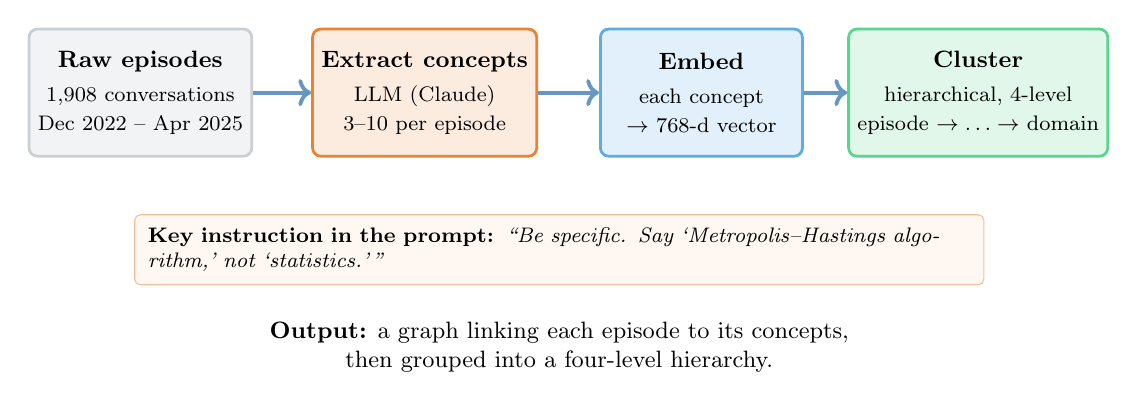
\begin{tikzpicture}[scale=0.95, transform shape,
        node distance=0.6cm,
        stage/.style={draw, rounded corners=3pt, minimum height=1.7cm, minimum width=2.7cm,
                      align=center, font=\small, line width=1pt},
        arrow/.style={->, line width=1.4pt, PrimaryBlue!60}]

        % Stage 1: raw episodes
        \node[stage, fill=ShadowGray!20, draw=ShadowGray!80] (raw) at (0, 0) {%
            \textbf{Raw episodes}\\[2pt]\footnotesize 1{,}908 conversations\\\footnotesize Dec 2022 -- Apr 2025};
        % Stage 2: concept extraction
        \node[stage, fill=AccentOrange!12, draw=AccentOrange!80] (ext) at (3.8, 0) {%
            \textbf{Extract concepts}\\[2pt]\footnotesize LLM (Claude)\\\footnotesize 3--10 per episode};
        % Stage 3: embedding
        \node[stage, fill=TheoreticalBlue!15, draw=TheoreticalBlue!80] (emb) at (7.5, 0) {%
            \textbf{Embed}\\[2pt]\footnotesize each concept\\\footnotesize $\to$ 768-d vector};
        % Stage 4: hierarchical clustering
        \node[stage, fill=PracticalGreen!15, draw=PracticalGreen!80] (cl) at (11.2, 0) {%
            \textbf{Cluster}\\[2pt]\footnotesize hierarchical, 4-level\\\footnotesize episode $\to \ldots \to$ domain};

        \draw[arrow] (raw) -- (ext);
        \draw[arrow] (ext) -- (emb);
        \draw[arrow] (emb) -- (cl);

        % Below: example concept extraction
        \node[draw=AccentOrange!40, fill=AccentOrange!5, rounded corners=2pt,
              text width=11cm, font=\footnotesize, align=left, inner sep=5pt]
              at (5.6, -2.1) {%
            \textbf{Key instruction in the prompt:}
            \emph{``Be specific. Say `Metropolis--Hastings algorithm,'
            not `statistics.'\,''}};

        % Output description (drops the cardinality preview so the
        % four-level reveal lands fresh on slide 5).
        \node[font=\small, align=center] at (5.6, -3.4) {%
            \textbf{Output:} a graph linking each episode to its concepts,\\
            then grouped into a four-level hierarchy.};
    \end{tikzpicture}

    \note{%
        \textbf{Slide 4 -- Pipeline (1:00, $\sim$120w)}\\[2pt]
        \textit{[Gesture along the pipeline arrows.]} Four stages.\\[2pt]
        \emph{Raw episodes}: 1{,}908 ChatGPT conversations over 29 months from one
        user --- me. Single-user case study; I'll come back to that.\\[2pt]
        \emph{Extract concepts}: an LLM pulls three to ten concepts from each
        episode. \textit{[Gesture: prompt box.]} The key detail is specificity.
        Not ``statistics''; ``Metropolis-Hastings algorithm.'' Specific concepts
        are what makes the geometry work later.\\[2pt]
        \emph{Embed}: each concept becomes a 768-dimensional vector.\\[2pt]
        \emph{Cluster}: hierarchical clustering, cut at three heights.\\[2pt]
        \textit{[Gesture: bottom output.]} The output is a graph linking episodes to
        concepts, plus a four-level hierarchy. Everything that follows is just
        \emph{measuring} this structure.\\[2pt]
        Here's what came out.
    }
\end{frame}

% =====================================================================
% 5. THE REVEAL -- 4-LEVEL HIERARCHY
% =====================================================================
\begin{frame}{The Reveal: A Four-Level Hierarchy Emerges}
    \begin{columns}[T]
        \column{0.55\textwidth}
        \centering
        % Clean 4-level cascade diagram (replaces unreadable sunburst).
        % Box widths encode level cardinality (1908 -> 500 -> 50 -> 8);
        % the right-column table names the 8 domains, so this figure
        % shows STRUCTURE rather than duplicating membership.
        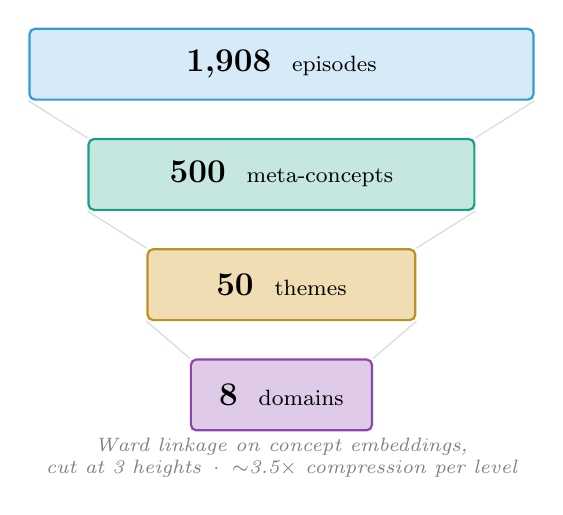
\begin{tikzpicture}[
            layer/.style={draw, thick, rounded corners=2pt, align=center,
                          minimum height=0.9cm, font=\footnotesize},
            branch/.style={ShadowGray, line width=0.5pt, opacity=0.55}
        ]
            \node[layer, fill=TheoreticalBlue!20, draw=TheoreticalBlue,
                  minimum width=6.4cm] (l1) at (0, 4.4)
                {\textbf{\large 1{,}908}\;\; episodes};
            \node[layer, fill=BridgeTeal!25, draw=BridgeTeal,
                  minimum width=4.9cm] (l2) at (0, 3.0)
                {\textbf{\large 500}\;\; meta-concepts};
            \node[layer, fill=NeoGold!35, draw=NeoGold!90!black,
                  minimum width=3.4cm] (l3) at (0, 1.6)
                {\textbf{\large 50}\;\; themes};
            \node[layer, fill=HippoPurple!28, draw=HippoPurple,
                  minimum width=2.3cm] (l4) at (0, 0.2)
                {\textbf{\large 8}\;\; domains};

            \draw[branch] (l1.south west) -- (l2.north west);
            \draw[branch] (l1.south east) -- (l2.north east);
            \draw[branch] (l2.south west) -- (l3.north west);
            \draw[branch] (l2.south east) -- (l3.north east);
            \draw[branch] (l3.south west) -- (l4.north west);
            \draw[branch] (l3.south east) -- (l4.north east);

            \node[font=\scriptsize\itshape, gray, align=center] at (0, -0.6)
                {Ward linkage on concept embeddings,\\ cut at 3 heights
                 \,$\cdot$\, $\sim$3.5$\times$ compression per level};
        \end{tikzpicture}

        \column{0.45\textwidth}
        \vspace{0.05cm}

        \textbf{Eight interpretable domains}

        \vspace{0.1cm}
        {\footnotesize
        \begin{tabular}{@{}l@{\hspace{6pt}}r@{}}
            Software Engineering & 1{,}074 \\
            Math \& Optimisation & 634 \\
            Statistical Methods & 510 \\
            Philosophy \& AI Theory & 489 \\
            ML \& Network Science & 274 \\
            DevOps \& Integration & 273 \\
            AI Safety \& Research & 177 \\
            LLM Engineering & 86 \\
        \end{tabular}
        }

        \vspace{0.15cm}

        \begin{exampleblock}{Two surprises}
            \footnotesize
            \begin{itemize}\setlength\itemsep{0.15em}
                \item Domains are \textbf{easy to name} --- but there's no clean number of clusters.
                \item Most episodes \textbf{belong to several domains at once}.
            \end{itemize}
        \end{exampleblock}

    \end{columns}

    \note{%
        \textbf{Slide 5 -- The Reveal (1:10, $\sim$145w)}\\[2pt]
        \textit{[Pause. Let the picture land.]}\\[2pt]
        \textit{[Gesture top to bottom along the cascade.]} 1{,}908 episodes consolidate
        into 500 meta-concepts, then 50 themes, then 8 domains. Each level groups
        roughly 3.5 of the level below --- the geometric signature of a hierarchy.\\[2pt]
        \textit{[Gesture: domain table.]} The eight domains are easy to name. I didn't
        pre-specify them. Software engineering largest, then math, statistics,
        philosophy of AI, ML and network science, devops, AI safety, LLM engineering.
        They reflect my actual research and project history.\\[2pt]
        \textit{[Gesture: ``Two surprises'' block.]} Two surprises.\\[2pt]
        \emph{First}: there's no clean number of clusters. Knowledge is a continuum,
        not a set of crisp categories. Eight domains is a useful summary, not a
        ``right answer.''\\[2pt]
        \emph{Second}: most episodes belong to several domains at once. We'll come
        back to that.\\[2pt]
        Cognitive science predicts two signatures here. Both have to land for the
        analogy to hold. Here's the first.
    }
\end{frame}

% =====================================================================
% 6. SMALL-WORLD TOPOLOGY
% =====================================================================
\begin{frame}{Signature 1: Small-World Topology}
    \begin{columns}[T]
        \column{0.55\textwidth}
        \centering

        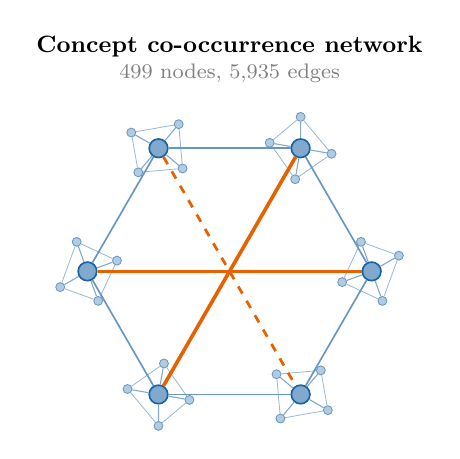
\begin{tikzpicture}[scale=0.95, transform shape]
            % Title
            \node[font=\small\bfseries] at (0, 3.0) {Concept co-occurrence network};
            \node[font=\footnotesize, gray] at (0, 2.65) {499 nodes, 5{,}935 edges};

            % Small-world cartoon: 6 dense local clusters around a ring,
            % with 3 long-range shortcuts crossing the centre.
            \begin{scope}[shift={(0, 0.0)}]
                \def\R{1.9}
                % For each of 6 cluster centres around a ring, draw a
                % dense local cluster of 4 nodes + a hub, all interconnected.
                \foreach \a/\name in {0/A, 60/B, 120/C, 180/D, 240/E, 300/F} {
                    \pgfmathsetmacro{\cx}{\R*cos(\a)}
                    \pgfmathsetmacro{\cy}{\R*sin(\a)}
                    % Hub
                    \node[circle, fill=PrimaryBlue!50, draw=PrimaryBlue!90,
                          inner sep=2.5pt, line width=0.6pt] (h\name) at (\cx, \cy) {};
                    % 4 satellites around the hub
                    \foreach \off/\sname in {30/s1, 110/s2, 200/s3, 290/s4} {
                        \pgfmathsetmacro{\sx}{\cx + 0.42*cos(\a+\off)}
                        \pgfmathsetmacro{\sy}{\cy + 0.42*sin(\a+\off)}
                        \node[circle, fill=PrimaryBlue!30, draw=PrimaryBlue!60,
                              inner sep=1.2pt, line width=0.3pt]
                              (\name\sname) at (\sx, \sy) {};
                        % Edge hub -> satellite (the local clustering)
                        \draw[PrimaryBlue!50, line width=0.4pt] (h\name) -- (\name\sname);
                    }
                    % Triangulate the satellites so each cluster looks dense
                    \draw[PrimaryBlue!40, line width=0.3pt] (\name s1) -- (\name s2);
                    \draw[PrimaryBlue!40, line width=0.3pt] (\name s2) -- (\name s3);
                    \draw[PrimaryBlue!40, line width=0.3pt] (\name s3) -- (\name s4);
                    \draw[PrimaryBlue!40, line width=0.3pt] (\name s4) -- (\name s1);
                }
                % Ring connections between adjacent hubs (locality)
                \foreach \a/\b in {A/B, B/C, C/D, D/E, E/F, F/A} {
                    \draw[PrimaryBlue!60, line width=0.6pt] (h\a) -- (h\b);
                }
                % Long-range shortcuts (small-world)
                \draw[AccentOrange, line width=1.3pt] (hA) -- (hD);
                \draw[AccentOrange, line width=1.3pt] (hB) -- (hE);
                \draw[AccentOrange, line width=1.0pt, dashed] (hC) -- (hF);
            \end{scope}
        \end{tikzpicture}

        \column{0.45\textwidth}
        \vspace{0.15cm}

        \textbf{Compared to a random graph}\\[-1pt]
        {\tiny\itshape\color{gray} [Humphries \& Gurney 2008]}

        \vspace{0.05cm}
        {\small
        \begin{tabular}{@{}lr@{}}
            \toprule
            Local clustering & $\mathbf{6.89\times}$ \\
            Shortest paths   & $1.05\times$ \\
            \midrule
            \textbf{Small-worldness} & $\mathbf{6.6}$ \\
            \bottomrule
        \end{tabular}}

        \vspace{0.15cm}

        \begin{block}{Matches human memory \textnormal{\itshape\footnotesize (small-worldness)}}
            \small
            \begin{tabular}{@{}lr@{}}
                Roget's Thesaurus   & $\approx 13$ \\
                WordNet             & $\approx 15$ \\
                Word associations   & $\approx 5.6$ \\
                \textbf{Our archive}        & $\boldsymbol{\approx 6.6}$ \\
            \end{tabular}\\[2pt]
            {\tiny\itshape\color{gray} [comparison values: Steyvers \& Tenenbaum 2005]}
        \end{block}
    \end{columns}

    \note{%
        \textbf{Slide 6 -- Small-World Topology (1:15, $\sim$130w)}\\[2pt]
        \textit{[Gesture: network cartoon.]} The concept co-occurrence network:
        499 meta-concepts as nodes, edges when concepts share an episode.\\[2pt]
        \textit{[Gesture: clusters, then orange shortcuts.]} Dense local clusters
        with a few long-range shortcuts. The Humphries-Gurney test compares
        clustering and path length against random graphs at matched size.\\[2pt]
        \textit{[Gesture: ratio table.]} Clustering 6.9 times higher than random.
        Path length essentially unchanged. Small-worldness of 6.6.\\[2pt]
        \textit{[Gesture: human-memory block.]} Roget's, WordNet, free-association
        norms give small-worldness between 5 and 15. The archive sits inside that
        range.\\[2pt]
        One caveat: I'm not claiming archives \emph{are} semantic memory. They show
        the same structural signature --- an externalised analog.\\[2pt]
        Signature one, confirmed. Now signature two: does the meta-concept layer
        consolidate the way CLS predicts?
    }
\end{frame}

% =====================================================================
% 7. HEAPS' LAW + NULL MODELS
% =====================================================================
\begin{frame}{Signature 2: Sublinear Vocabulary Growth}
    \begin{columns}[T]
        \column{0.62\textwidth}
        \centering
        % Slide-optimized single-panel version with both null bands shown,
        % cleaner legend (no V(n)=K*n^beta entries). See:
        % experiments/figures/generate_heaps_law_slide.py
        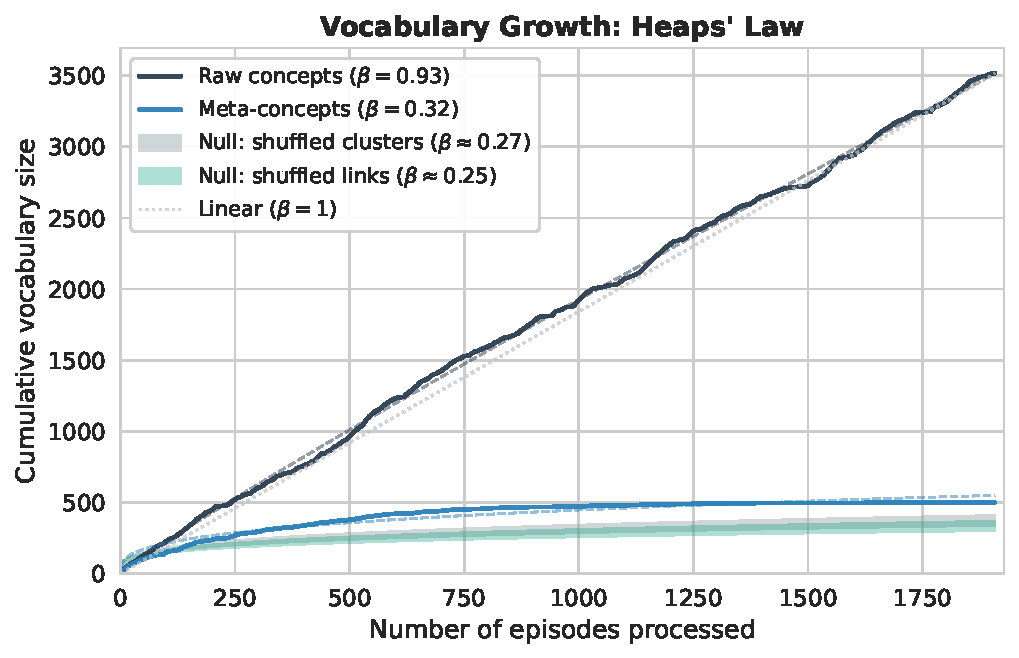
\includegraphics[width=\textwidth, height=0.78\textheight, keepaspectratio]{heaps_law_slide.pdf}

        \column{0.38\textwidth}
        \vspace{0.05cm}

        \textbf{Heaps' law: $V(n) = K \cdot n^{\beta}$}\\
        {\tiny\itshape\color{gray} [Heaps 1978]}

        \vspace{0.1cm}
        {\footnotesize
        \begin{tabular}{@{}lr@{}}
            \toprule
            Raw concepts          & $\beta = 0.93$ \\
            \textbf{Meta-concepts} & $\boldsymbol{\beta = 0.32}$ \\
            \bottomrule
        \end{tabular}}

        \vspace{0.15cm}

        \begin{alertblock}{Caveat: with $k$ fixed at 500}
            \footnotesize
            Some saturation is automatic. So we compare against \textbf{null models}.
        \end{alertblock}

        \vspace{0.1cm}

        \begin{exampleblock}{Two nulls, both reject}
            \footnotesize
            \begin{itemize}\setlength\itemsep{0.1em}
                \item Shuffled clusters: $\beta = 0.27$
                \item Shuffled links: $\beta = 0.25$
                \item Both $p < 10^{-3}$
            \end{itemize}
        \end{exampleblock}
    \end{columns}

    \vspace{0.1cm}

    \centering
    \footnotesize
    \textcolor{PrimaryBlue!80}{\textbf{Observed $\beta$ is \emph{higher} than either null}:
    coherent categories require novel territory to add a new label.}

    \note{%
        \textbf{Slide 7 -- Vocabulary saturates (1:15, $\sim$135w)}\\[2pt]
        \textit{[Gesture: plot.]} Heaps' law: vocabulary grows like $n^\beta$.
        Real text has $\beta$ around 0.4 to 0.6. Lower means stronger saturation
        --- the consolidation CLS predicts.\\[2pt]
        \textit{[Gesture: top curve.]} Raw concepts grow nearly linearly,
        $\beta = 0.93$. We keep inventing new noun phrases. \textit{[Gesture:
        bottom curve.]} Meta-concepts: $\beta = 0.32$. Strongly sublinear.\\[2pt]
        \textit{[Gesture: caveat.]} But fixing the number of clusters at 500 means
        some saturation is automatic. We need null models.\\[2pt]
        \textit{[Gesture: two-nulls block.]} First null: shuffle which raw concept
        goes in which cluster. $\beta = 0.27$. Second null: shuffle the
        episode-concept links while keeping the row and column totals.
        $\beta = 0.25$. Our $0.32$ exceeds both at $p < 10^{-3}$.\\[2pt]
        Why \emph{higher}, not lower? Coherent clusters draw real distinctions;
        random clusters absorb anything. The saturation is real --- and it only
        showed up because we kept the set-based structure. Which is the next slide.
    }
\end{frame}

% =====================================================================
% 8. THE BIPARTITE ADVANTAGE -- BRIDGE
% =====================================================================
\begin{frame}{77\% of Episodes Span Multiple Domains}
    \centering
    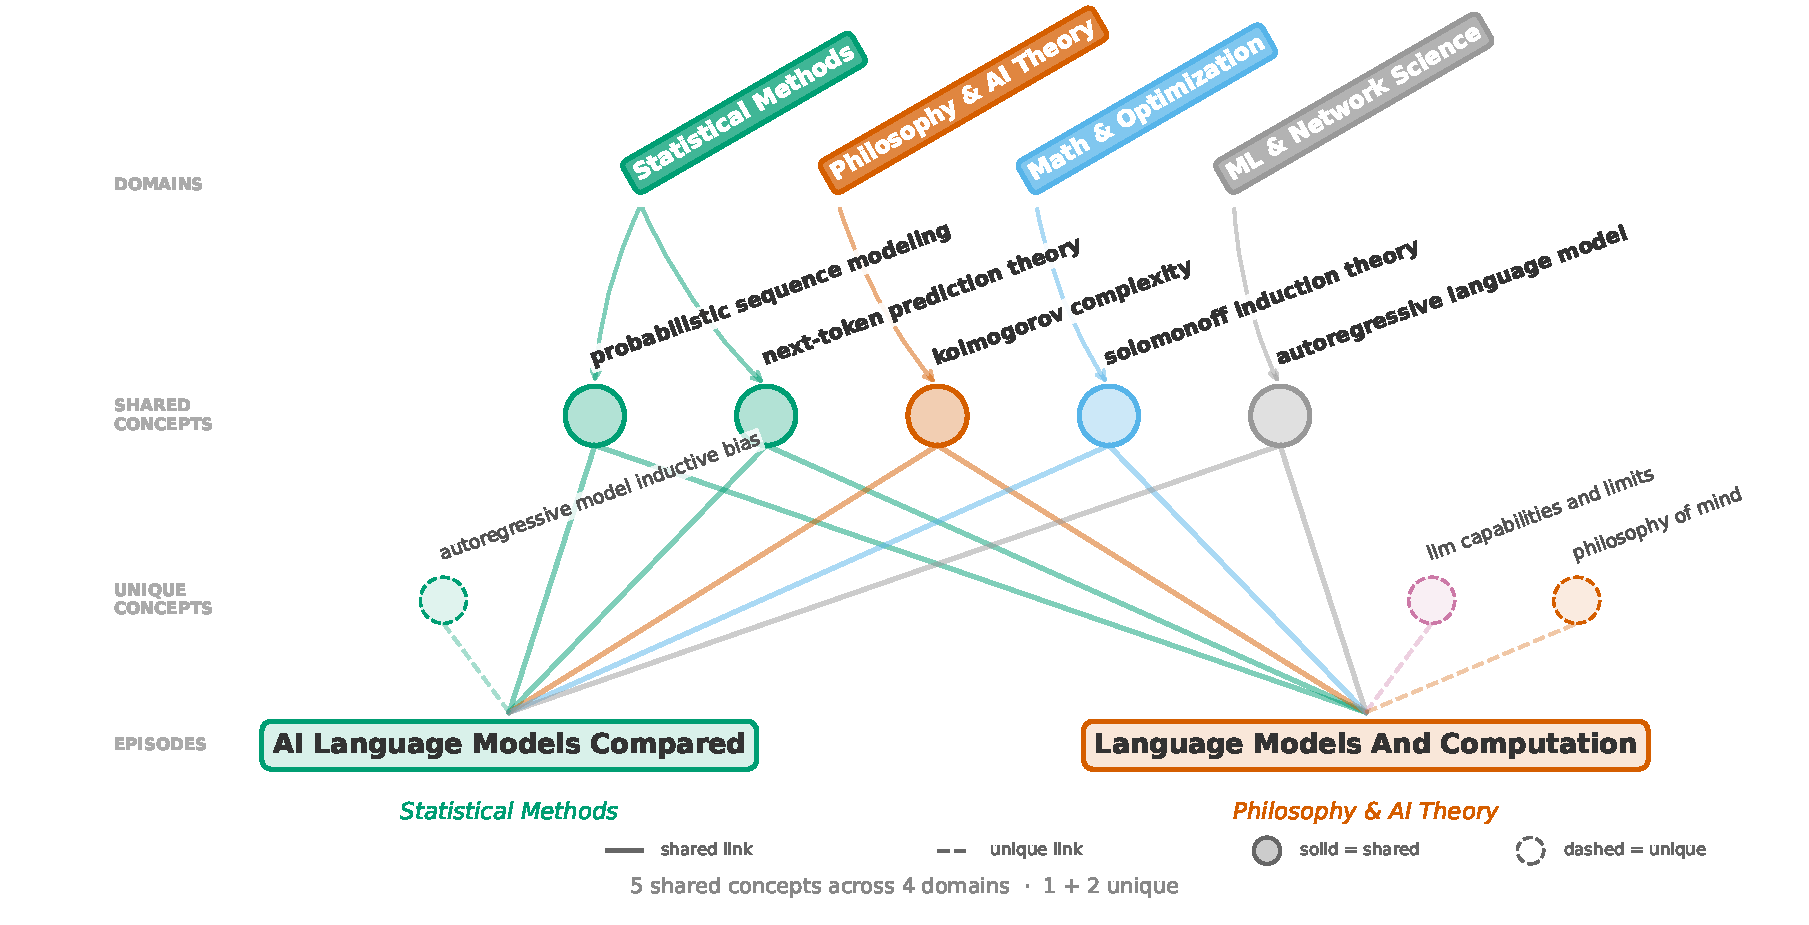
\includegraphics[width=0.95\textwidth, height=0.66\textheight, keepaspectratio]{zoom_in_bridge.pdf}

    \vspace{0.05cm}

    \begin{columns}[T]
        \column{0.52\textwidth}
        \footnotesize
        \textbf{One-label methods} \textit{(Louvain, $k$-means, BERTopic)}: each
        episode gets one cluster. These two end up apart --- connection vanishes.

        \column{0.48\textwidth}
        \footnotesize
        \textbf{Set-based methods}: each episode is a \emph{set} of concepts.
        Two episodes share concepts across \emph{four} domains and stay linked.
    \end{columns}

    \note{%
        \textbf{Slide 8 -- 77\% span multiple domains (1:10, $\sim$125w)}\\[2pt]
        \textit{[Gesture: the two episode boxes.]} Two real episodes. One lives in
        Statistical Methods. The other lives in Philosophy and AI Theory. Different
        domains.\\[2pt]
        \textit{[Gesture: the shared concept list in the middle.]} But they share
        five concepts --- Kolmogorov complexity, Solomonoff induction, and three
        others --- and those five concepts span \emph{four} different domains.\\[2pt]
        Any one-label-per-episode method assigns each episode to a single cluster.
        These two episodes end up in different clusters and the connection
        \emph{vanishes}.\\[2pt]
        The set-based model preserves it. An episode \emph{is} a set of concepts; two
        episodes link through any shared concept, regardless of which domain that
        concept lives in.\\[2pt]
        And this isn't rare: \textbf{77\% of episodes span two or more domains;
        35\% span three or more.} Cross-domain is the rule. That's the
        methodological contribution.\\[2pt]
        With this structure, we can ask a question single-label methods can't.
    }
\end{frame}

% =====================================================================
% 9. ASYMMETRIC FLOW
% =====================================================================
\begin{frame}{Who Borrows From Whom? (Concept Flow)}
    \begin{columns}[T]
        \column{0.60\textwidth}
        \centering
        % Trim right panel (broadcast/porosity bar chart): right column
        % covers reach + porosity verbally. Keeping just the heatmap
        % makes the percentages and domain labels readable.
        % Native page: 1047 x 496 pts.
        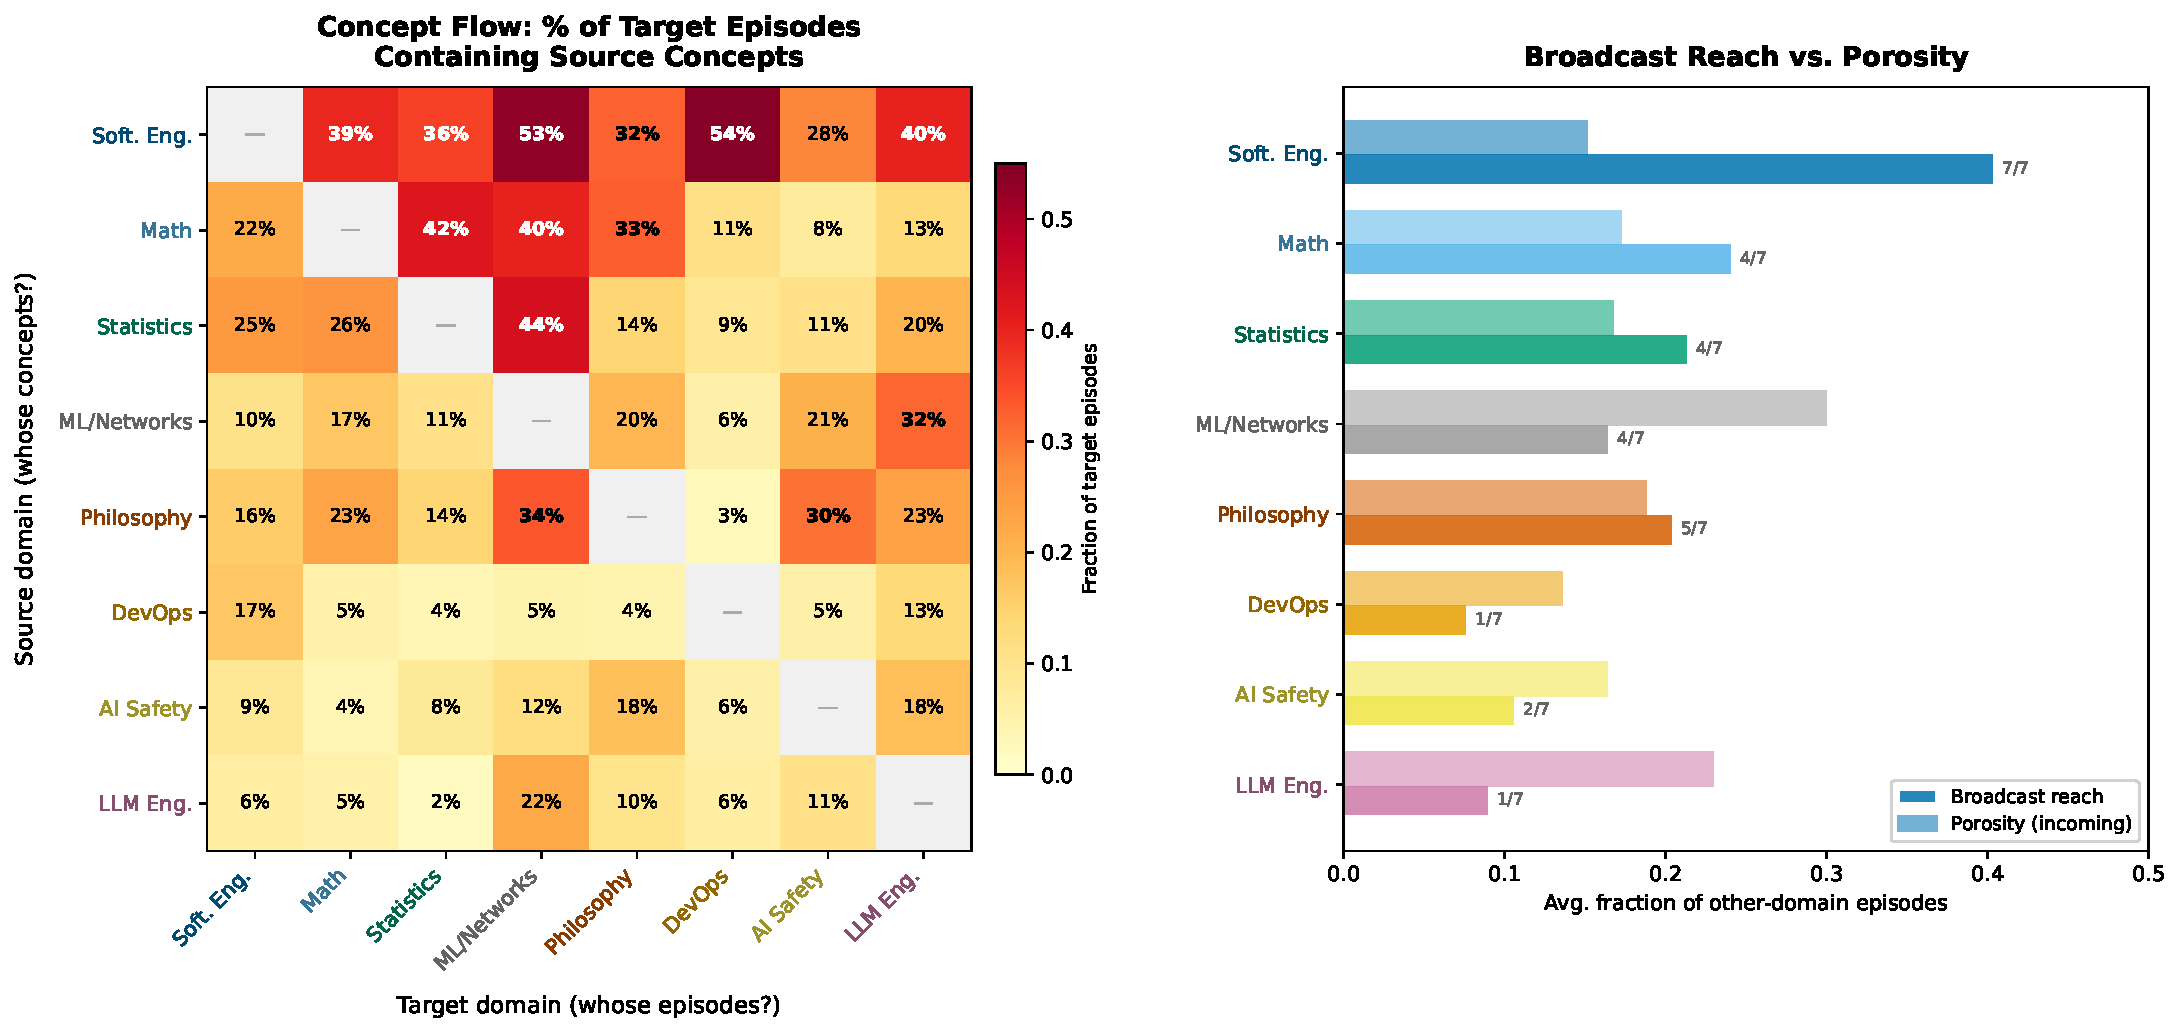
\includegraphics[width=\textwidth, height=0.82\textheight, keepaspectratio,
                         trim=0 0 500 0, clip]{domain_flow.pdf}

        \column{0.40\textwidth}
        \vspace{0.05cm}

        \textbf{Two questions per domain}

        \vspace{0.1cm}
        {\footnotesize \textcolor{PrimaryBlue}{\textbf{Where do its concepts go?}} (rows)}\\[0.1cm]
        {\footnotesize \textcolor{AccentOrange}{\textbf{Which concepts come in?}} (columns)}

        \vspace{0.2cm}

        \begin{block}{What the heatmap says}
            \footnotesize
            \begin{itemize}\setlength\itemsep{0.25em}
                \item On average \textbf{39\% below} random\\ $\Rightarrow$ domains really are separate
                \item LLM Eng.\ $\to$ ML/Net: \textbf{2.67$\times$} random\\ $\Rightarrow$ specific dependencies
            \end{itemize}
        \end{block}

        \vspace{0.1cm}
        {\footnotesize \textit{Software Eng.\ broadcasts to all 7 others.}}
    \end{columns}

    \note{%
        \textbf{Slide 9 -- Who borrows from whom (1:10, $\sim$135w)}\\[2pt]
        \textit{[Gesture: heatmap.]} For each pair of domains $(A,B)$: what fraction
        of $B$'s episodes contain a concept from $A$? Reading across a row tells you
        where $A$'s concepts go. The reverse direction is usually different ---
        asymmetry an undirected network can't see.\\[2pt]
        \textit{[Trace Software Engineering's row.]} Software Engineering broadcasts
        into every other domain. \textit{[Gesture: math$\leftrightarrow$statistics.]}
        Math and statistics feed each other heavily. \textit{[Gesture: LLM Eng.\ row.]}
        LLM Engineering is small but punches above its weight.\\[2pt]
        The catch: Software Engineering owns 30\% of raw concepts. Are we just
        measuring size? We control against a null that shuffles concept--domain
        labels while keeping the sizes fixed.\\[2pt]
        On average, sharing comes in \textbf{39\% below random}. Domains really are
        separate.\\[2pt]
        \textit{[Gesture: heatmap-says block.]} But specific pipelines stand out.
        LLM Engineering $\to$ ML and Networks: \textbf{2.67$\times$} the random
        expectation. That's a targeted dependency, not spillover.\\[2pt]
        The story: \emph{real boundaries, with a few specific pipelines}.\\[2pt]
        Here's what the whole thing looks like.
    }
\end{frame}

% =====================================================================
% 10. THE FULL KNOWLEDGE MAP
% =====================================================================
\begin{frame}{The Full Picture}
    \centering
    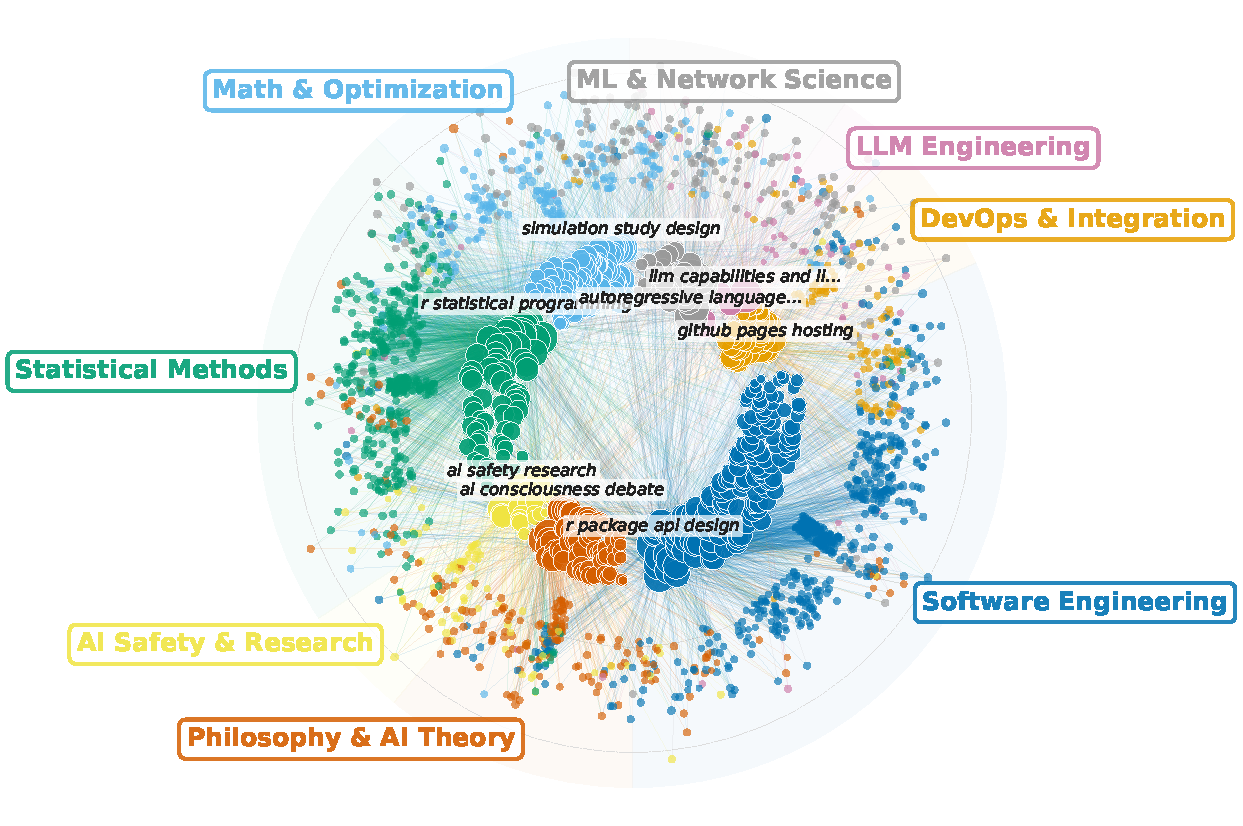
\includegraphics[width=0.82\textwidth, height=0.80\textheight, keepaspectratio]{knowledge_map_bipartite.pdf}

    {\scriptsize\textit{Inner: 499 concepts (coloured by domain). \ Outer: 1{,}908 episodes. \ Edges: episode$\to$concept.}}

    \note{%
        \textbf{Slide 10 -- The Full Picture (35 s, $\sim$70w)}\\[2pt]
        \textit{[Gesture: the whole image; caption already names the rings.]} The
        whole archive in one image.\\[2pt]
        \textit{[Trace Software Engineering's sector.]} Software Engineering sends
        links everywhere. \textit{[Gesture to Philosophy.]} Philosophy and AI Theory
        stays mostly within its own sector. Statistics, math, AI safety, the small
        LLM sliver --- each visible as a distinct coloured region.\\[2pt]
        \textit{[Pause for the gestalt.]}\\[2pt]
        Three takeaways.
    }
\end{frame}

% =====================================================================
% 11. CONCLUSIONS
% =====================================================================
\begin{frame}{Takeaways \& What's Next}
    \begin{columns}[T]
        % COL 1: WHAT WE FOUND (narrower side panel)
        \column{0.30\textwidth}
        \begin{exampleblock}{What we found}
            \footnotesize
            \begin{itemize}\setlength\itemsep{0.25em}
                \item 4-level hierarchy\\ 1{,}908 $\to$ 500 $\to$ 50 $\to$ 8
                \item Small-world structure\\ matches human memory
                \item Vocabulary saturates\\ as CLS predicts
                \item 77\% span $\geq 2$ domains
            \end{itemize}
        \end{exampleblock}

        % COL 2: WHY IT MATTERS -- centerpiece (wider + larger font)
        % This is the column the audience walks away repeating, so it
        % visually dominates: 40% width and \small instead of \footnotesize.
        \column{0.40\textwidth}
        \begin{block}{Why it matters}
            \small
            \begin{itemize}\setlength\itemsep{0.35em}
                \item Archives = \textbf{externalised semantic memory}
                \item Natural index for \textbf{concept-level Graph~RAG}
                \item Knowledge is a \textbf{continuum, not a partition}
            \end{itemize}
        \end{block}

        % COL 3: LIMITS & NEXT (narrower side panel)
        \column{0.30\textwidth}
        \begin{alertblock}{Limits \& next}
            \footnotesize
            \begin{itemize}\setlength\itemsep{0.25em}
                \item \textbf{N=1} single user.\\ Replicate on WildChat
                \item No natural $k$
                \item Extend to \textbf{agentic} sessions
            \end{itemize}
        \end{alertblock}
    \end{columns}

    \vspace{0.2cm}

    \centering
    \begin{tcolorbox}[colback=PrimaryBlue!5, colframe=PrimaryBlue!40, boxrule=0.6pt,
                       arc=2pt, left=8pt, right=8pt, top=3pt, bottom=3pt, width=0.88\textwidth]
        \centering
        \small
        Treat AI conversation archives as \textbf{structured cognitive artifacts} ---\\
        the structure was there all along; we just needed the right lens.
    \end{tcolorbox}

    \vspace{0.1cm}
    \centering
    \footnotesize \textcolor{PrimaryBlue}{\textbf{Questions?}} \quad
    \faGithub\ \texttt{queelius/chatgpt-complex-net}

    \note{%
        \textbf{Slide 11 -- Takeaways (1:10, $\sim$155w)}\\[2pt]
        Three angles to take away.\\[2pt]
        \textit{[Gesture: ``What we found'' column.]} Four-level hierarchy: 1{,}908
        episodes, 500 concepts, 50 themes, 8 domains. Small-world structure matching
        human-memory benchmarks. Vocabulary saturates, as CLS predicts. And most
        episodes span multiple domains.\\[2pt]
        \textit{[Gesture: ``Why it matters'' column.]} A principled way to treat AI
        archives as externalised semantic memory. A natural index for concept-level
        retrieval over your own conversations. And: knowledge is a continuum, not a
        partition.\\[2pt]
        \textit{[Gesture: ``Limits and next'' column.]} N equals one --- next step is
        replicating on WildChat. No natural number of clusters. And we're extending
        the method to \emph{agentic} sessions, where parent-child delegation adds a
        layer.\\[2pt]
        \textit{[Gesture: bottom takeaway box.]} The headline: treat AI conversation
        archives as structured cognitive artifacts. The structure was there all
        along; we just needed the right lens.\\[2pt]
        Thank you. Code and data at the link. Happy to take questions.
    }
\end{frame}

% =====================================================================
% BACKUP: METHOD DETAILS
% =====================================================================
\begin{frame}[noframenumbering]{Backup: Method Details}
    \begin{columns}[T]
        \column{0.5\textwidth}
        \textbf{Concept extraction}
        \begin{itemize}
            \footnotesize
            \item Model: \texttt{claude-3-5-sonnet-20241022}, T=0
            \item Per episode: first 20 messages, 500-char cap
            \item Target: 3--10 noun phrases, 2--5 words
            \item 20 parallel agents (no shared vocabulary)
            \item Post-hoc dedup: geometric (no string matching)
        \end{itemize}

        \vspace{0.2cm}

        \textbf{Embedding}
        \begin{itemize}
            \footnotesize
            \item Model: \texttt{nomic-embed-text}
            \item 768-dim, 8k context, L2-normalised
        \end{itemize}

        \column{0.5\textwidth}
        \textbf{Hierarchical clustering}
        \begin{itemize}
            \footnotesize
            \item Ward linkage, Euclidean distance
            \item Cuts at $k = 500, 50, 8$
            \item Silhouette monotonic for $k \geq 20$ (no natural boundaries)
        \end{itemize}

        \vspace{0.2cm}

        \textbf{Yield}
        \begin{itemize}
            \footnotesize
            \item 7{,}555 raw concept mentions
            \item 3{,}517 unique (after case dedup)
            \item 500 meta-concepts after Ward
            \item 7{,}153 bipartite edges
            \item 5{,}935 co-occurrence edges on 499 nodes
        \end{itemize}
    \end{columns}
\end{frame}

% =====================================================================
% BACKUP: SENSITIVITY
% =====================================================================
\begin{frame}[noframenumbering]{Backup: Robustness to $k$}
    \centering

    \begin{tabular}{rrrrr}
        \toprule
        $k$ & Heaps' $\beta$ & Small-worldness & Clustering $C$ & Edges \\
        \midrule
        50   & 0.061 &  1.1 & 0.830 &    906 \\
        100  & 0.103 &  1.4 & 0.652 &  2{,}286 \\
        200  & 0.158 &  2.0 & 0.425 &  4{,}111 \\
        300  & 0.225 &  2.9 & 0.351 &  5{,}073 \\
        \textbf{500} & \textbf{0.320} & \textbf{6.57} & \textbf{0.329} & \textbf{5{,}935} \\
        700  & 0.382 & 12.6 & 0.351 &  6{,}593 \\
        1000 & 0.467 & 25.9 & 0.401 &  7{,}291 \\
        \bottomrule
    \end{tabular}

    \vspace{0.4cm}

    \begin{block}{}
        \footnotesize
        \centering
        \emph{Qualitative} conclusions (small-worldness $> 1$, sublinear $\beta$, null rejection)
        hold for every $k$ tested.\\
        \emph{Quantitative} numbers shift smoothly: the 500-cluster cut is a useful summary,
        not a privileged scale.
    \end{block}
\end{frame}

\end{document}
